%%%%%%%%%%%%%%%%%%%%%%% file moduleX_template.tex %%%%%%%%%%%%%%%%%
%
%
% This is a template for creating your papers for the course KRW
% It is based on the standard Latex template for Springer publications
% but contains a suggestion for the structure and some content of the
% paper.
%
% Please adapt this document wherever needed.
%
% For more information about the required Latex Style check the document
% typeinst.pdf in the StyleFiles directory.
%
%%%%%%%%%%%%%%%%%%%%%%%%%%%%%%%%%%%%%%%%%%%%%%%%%%%%%%%%%%%%%%%%%%%%%%%%%


\documentclass[runningheads,a4paper]{../../StyleFiles/llncs}

\usepackage{url}
\usepackage{graphicx}
\usepackage{amssymb}


\newcommand{\keywords}[1]{\par\addvspace\baselineskip
\noindent\keywordname\enspace\ignorespaces#1}

\begin{document}

\mainmatter  % start of an individual contribution

% first the title is needed
\title{Ontology Matching Paper}

% a short form should be given in case it is too long for the running head
\titlerunning{Ontology Matching Paper}

% the name(s) of the author(s) follow(s) next
%
% NB: Chinese authors should write their first names(s) in front of
% their surnames. This ensures that the names appear correctly in
% the running heads and the author index.
%
\author{Alivanistos, Dimitris. \\ Baez, Selene. \\ Jemmett, Andrea.}
%
\authorrunning{Alivanistos, Dimitris. \\ Baez, Selene. \\ Jemmett, Andrea.}
% (feature abused for this document to repeat the title also on left hand pages)

% the affiliations are given next; don't give your e-mail address
% unless you accept that it will be published
\institute{\url{d.alivanistos@student.vu.nl} \and \url{s.baezsantamaria@student.vu.nl} \and \url{a.jemmett@student.vu.nl}}

\maketitle


\begin{abstract}
The abstract should summarize the contents of the paper and should
contain at least 70 and at most 150 words. It should be written using the
\emph{abstract} environment.
\end{abstract}


\section{Introduction}
%Introduce the sections that follow. What is the problem this paper addresses? What is the core contribution of this paper, and why is that interesting? What method did you develop and implement? What is the research question or hypothesis this paper answers? How did you answer this question or validate your approach (empirically, analytically). You might want to give a brief (qualitative) sketch of the results. 
In this paper we continue the work related for creating an application for finding Handicap Parking Spots close to Event Venues in Amsterdam. In the previous paper, we improved on the ontology to comply with the Five Star model and linked it to other existing ontologies. In this paper, we continue the work by matching and aligning the ontology to other subject-related ontologies. 

In general, the problem of matching ontologies has been studied before by Semantic Web researchers. As Shvaiko et al. state, the problem of heterogeneity is still a challenge to be solved since ambiguity in meanings and interpretations prevent us from finding equivalences in same domain ontologies \cite{shvaiko2013ontology}. Ontology matching and alignment allow to merge, translate, and extend ontologies, finding correspondences both in entities, properties and instances. The Ontology Alignment Evaluation Initiative is an annual international competition that serves as an evaluation for state of the art alignment tools. 

With that in mind, in this paper we select relevant vocabularies from the pool of Amsterdam related ontologies in our class. After some comparison we selected Group 10 -an ontology for cultural activities-, Group 13 -an ontology about safety for tourists using statistical area information-, and Group 15 -an ontology for general activity finding.

In the following sections we first revise existing tools for matching and aligning ontologies. Then we select and apply tools for matching and aligning our ontologies to the aforementioned ones, experimenting with different comparators. We continue to evaluate such algorithms and discuss the results. Finally, we conclude by summarizing the findings of the alignment to different ontologies.

\section{Related Work}
%Give here an overview over related matching methods and how they related to your own solution. Cite papers that might have inspired your approach. Sometimes it makes sense to have this section immediately after the introduction.
In order to match our ontology to others, we did research about state of the art matching and alignment tools. \cite{adaptiveInformation_2014} is a comprehensive list of the top 50 tools, separating active from inactive tools. Additionally, we looked at some of the tools revised by Euzenat et Al \cite{euzenat2007ontology}. Furthermore, we looked at the participants from the most recent OAEI.

In the following we list the most relevant tools.

\begin{enumerate}
	\item \textbf{OLA \cite{euzenat2004ontology}:} Developed in 2004, the OWL Lite Alignment (OLA) is a tool for automatic matching of ontologies that implements the OLA algorithm designed in collaboration by the DIRO, University of Montréal and INRIA Rhône Alpes. It participated in OEIA 2005 \cite{euzenat2005ola} and 2007 \cite{djoufak2007ola} and increased its own results from 0.80 to 0.89 in Precision, and 0.74 to 0.87 in Recall. At the time, it was one of the pioneers of ontology matching, yet no it is nowadays outdated.
	\item \textbf{S-Match \cite{giunchiglia2004s}:} S-Match is a semantic matching tool that is suitable for many applications. However, it is not specific for ontology matching and it has not participated in the latest OAEI.
	\item \textbf{MapONTO \cite{an2004refining}:} MapOnto, just as S-Match, is a general purpose semantic matcher. It is an Initiative from the University of Toronto and it is implemented as a plug-in for Protege. At first sight, this option seemed promising, however the latest release is compatible with obsolete versions of Protege. 
	%\item \textbf{WordNet:Similarity \cite{pedersen2004wordnet}:} Semantic 
	\item \textbf{AML \cite{faria2013agreementmakerlight}:} The Agreement
	Maker Light (AML) is the improved version of the original Agreement Maker. It is a simple, user-friendly application for matching ontologies which also provides visualization and evaluation of the alignment. Further details will be discussed in Section \ref{Ontology_Matching}.
\end{enumerate}

\section{Methods, Algorithms and Implementation}
% Introduce your method, i.e. the overall approach taken and the general idea, the\bibliography{paper}
 algorithms in general, maybe in pseudo-code and give a quick overview over the technical implementations (not too much details).

% Maybe you want to separate this part into subsections for your two systems
\subsection{Ontology Matching}
\label{Ontology_Matching}
- Decided to use one of the best candidates in the OAEI of 2014, AML (AgreementMakerLight) the best system (as measured in terms of F-measure) for lightweight ontologies. The reasons behind this choice was that AML exceeded our expectations with regard to run time results, comprehensive user interface and integrated evaluation mechanism. The procedure can be fully or semi automatic, with the user being presented to a fully customizable matching. We can choose between different metrics with respect to structure,content etc 
-examples with pictures, String Matcher, Word matcher, Property matcher, Cardinality matcher and background knowledge matcher.

\begin{figure}[h]\centering
	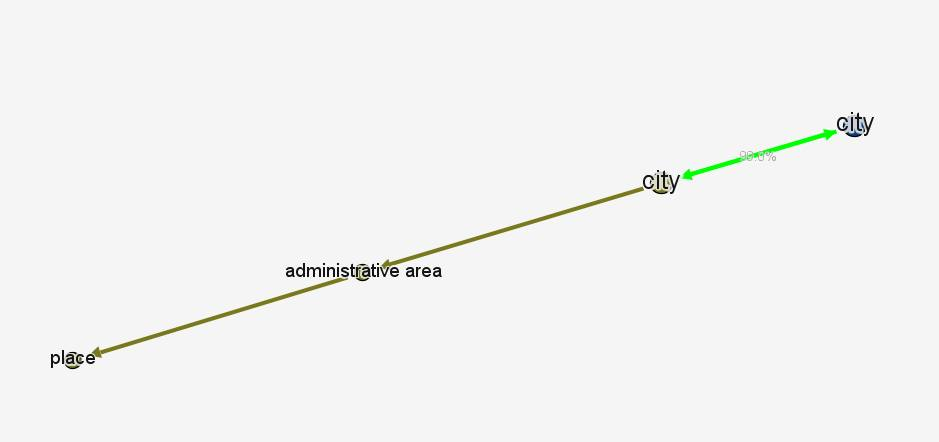
\includegraphics[width=.75\textwidth]{img/match_city.png}
	\caption{Visual representation of a single correct match in AML.}
	\label{fig:single_match}
\end{figure}
\begin{figure}[h] \centering
	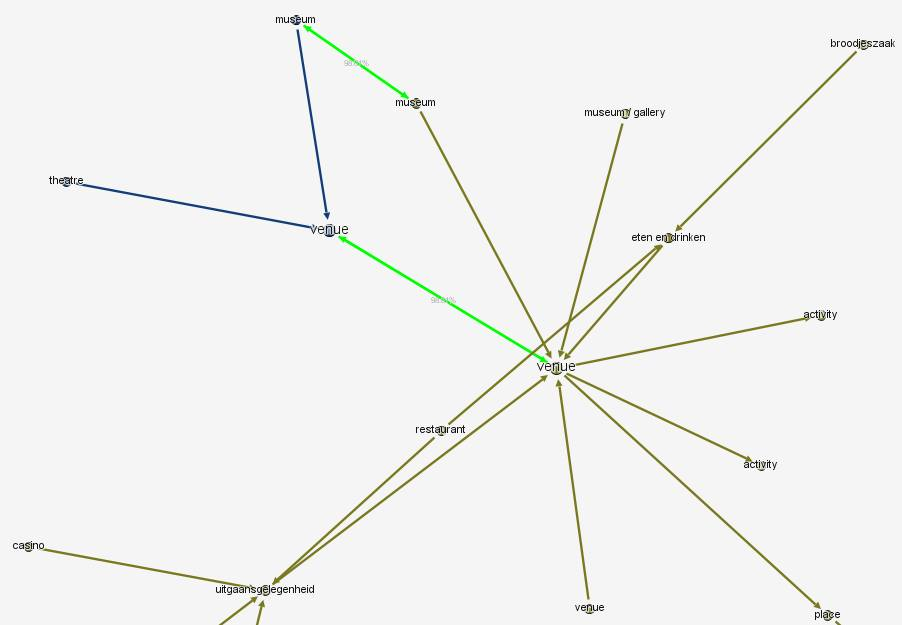
\includegraphics[width=.75\textwidth]{img/match_combo.png}
	\caption{Visual representation of multiple correct matches in AML.}
	\label{fig:multiple_match}
\end{figure}
\begin{figure}[h] \centering
	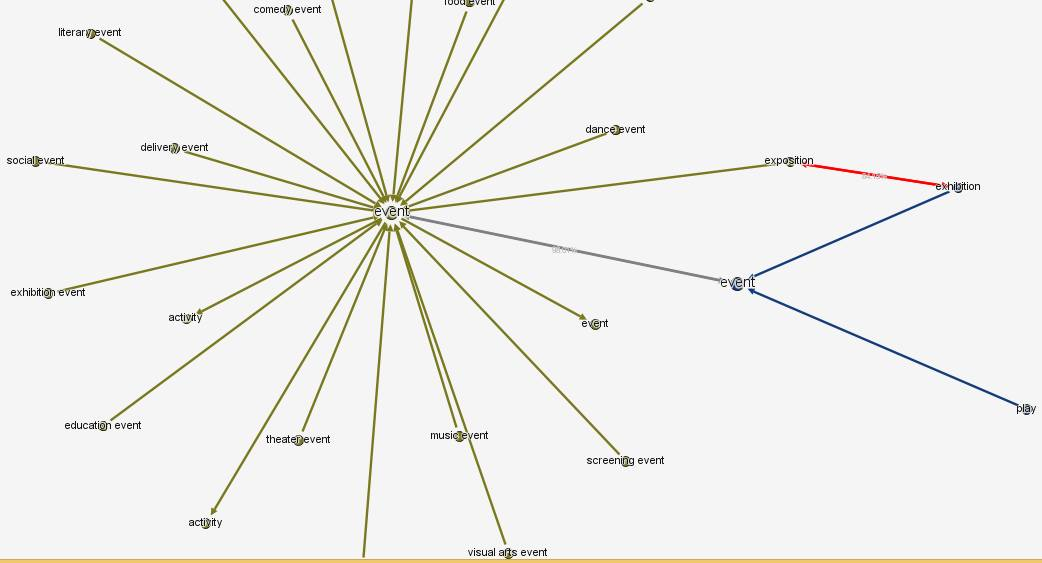
\includegraphics[width=.75\textwidth]{img/conflict_exhibition_exposition.png}
	\caption{Visual representation of an incorrect match in AML.}
	\label{fig:incorrect_match}
\end{figure}

\subsection{Data Linkage}
In this section the developed Data Linkage system is presented.
It interlinks our dataset with two other datasets from groups 13 and 15. We
decided to implement the linking workflow and procedures using the
\textit{Silk framework}\footnote{\url{http://silkframework.org/}} which captions
itself as ``The Linked Data Integration Framework''. Silk is an open source
project for integrating heterogeneous data sources and among its use cases is
generating links between Linked Data sources, which is exactly within our needs.
Moreover Silk provides the user with a nice and friendly Web-based GUI and a visual
editor for linkage rules.

To link two Linked Datasets using Silk first we need to define their sources,
e.g. using a SPARQL endpoint or uploading an RDF dump. Then it is possible to
create linkage rules by applying four different kind of operations:
\begin{enumerate}
	\item path-like queries to retrieve values;
	\item transformations over those values (e.g. to-lowercase, tokenization);
	\item comparators over values (e.g. Levenshtein distance, Jaccard
		coefficient, equality);
	\item aggregators over comparators output (e.g. average, minimum, maximum).
\end{enumerate}
It is also possible to specify a threshold for the comparator's output score,
its weight when computing an aggregation for it or whether it is required that a
value exists for that block\footnote{We say block because Silk uses a visual
editor with block-shaped functionalities.}.

\subsubsection{Linking the Cultural Dataset}
This dataset has a domain in part similar to our so the linking procedure
is trivial and reduces to a check on the \texttt{rdfs:label} and some other
property. An example Silk linkage rule is shown in Figure \ref{fig:link_event_g10}
that matches events; in this case the match is checked against
\texttt{rdfs:label} and \texttt{dc:title}.
%TODO link other entities

\begin{figure}[h]
	\centering
	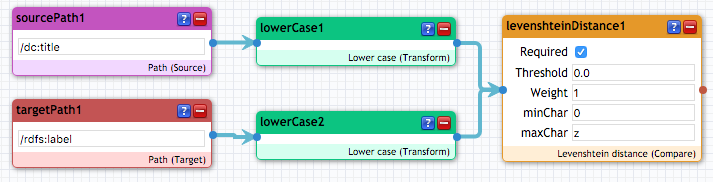
\includegraphics[width=1\textwidth]{img/link_event_g10.png}
	\caption{Silk linkage rules for events in group 10's dataset.}
	\label{fig:link_event_g10}
\end{figure}

\subsubsection{Linking the Tourist Safety Dataset}
In spite being about a different domain, this dataset can still be linked with
ours for what concerns events and locations / venues. Indeed the overlap between
events in this dataset and ours is big and we are able to match a big proportion
of entities by using a linkage rule similar to that shown in Figure
\ref{fig:link_event_g10} but using \texttt{rdfs:label} for both data sources.

\subsubsection{Linking the Activity Finding Dataset}
For events the linkage rule is less trivial and immediate than that for the
Cultural Dataset and involves the use of more properties and an aggregator as
shown in Figure \ref{fig:link_event_g15}.

\begin{figure}[h]
	\centering
	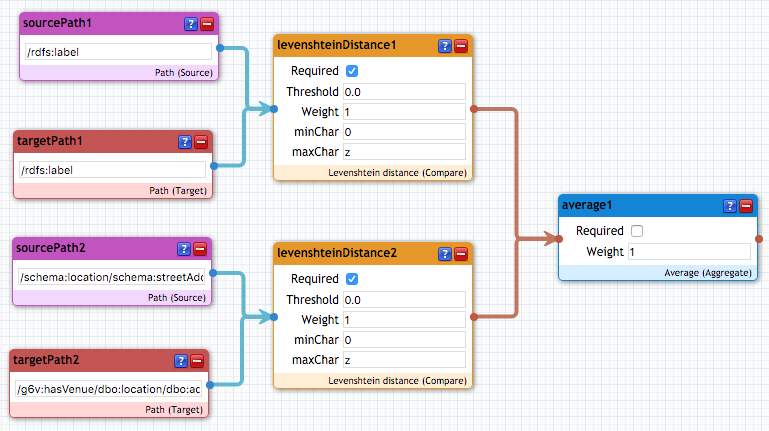
\includegraphics[width=1\textwidth]{img/link_event_g15.png}
	\caption{Silk linkage rule for events in the Activity Finding Dataset.
		\texttt{sourcePath2} contains
		\texttt{/schema:location/schema:streetAddress} while
		\texttt{targetPath2} contains
		\texttt{/g6v:hasVenue/dbo:location/dbo:address}.}
	\label{fig:link_event_g15}
\end{figure}


\section{Validation and Experiments}
% In a scientific paper you want to show that your choice of method and algorithms was the right choice. So, this could be a place where you make claims or ask concrete and explicit research questions (e.g. with respect to runtime and/or precision/recall.

\subsection{Group 10: Cultural Ontology}
We match to the main entities of Events and Venues.

\begin{figure}[h]\centering
	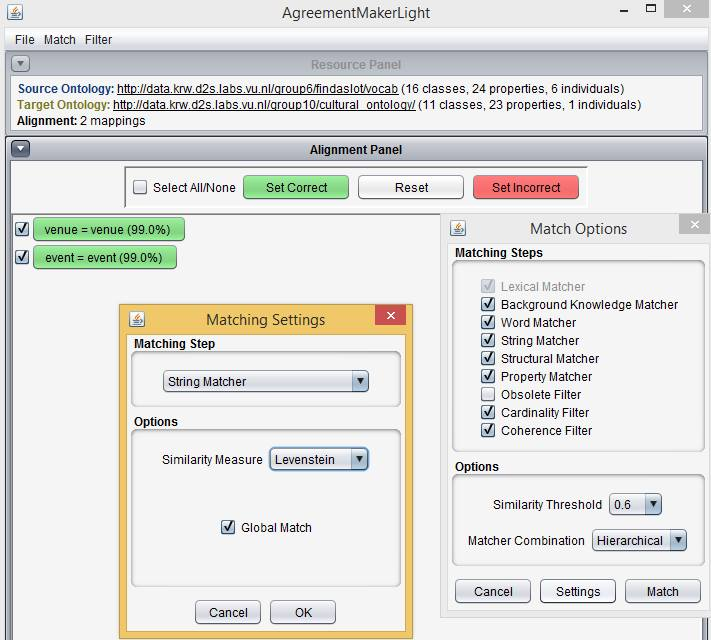
\includegraphics[width=.75\textwidth]{img/match_g10.png}
	\caption{Matching to group 10}
	\label{fig:match_g10}
\end{figure}

\subsection{Group 13: Tourist safety Ontology}


\subsection{Group 15: Activity finding Ontology}
Six correct matchings versus six incorrect matchings

\begin{figure}[h]\centering
	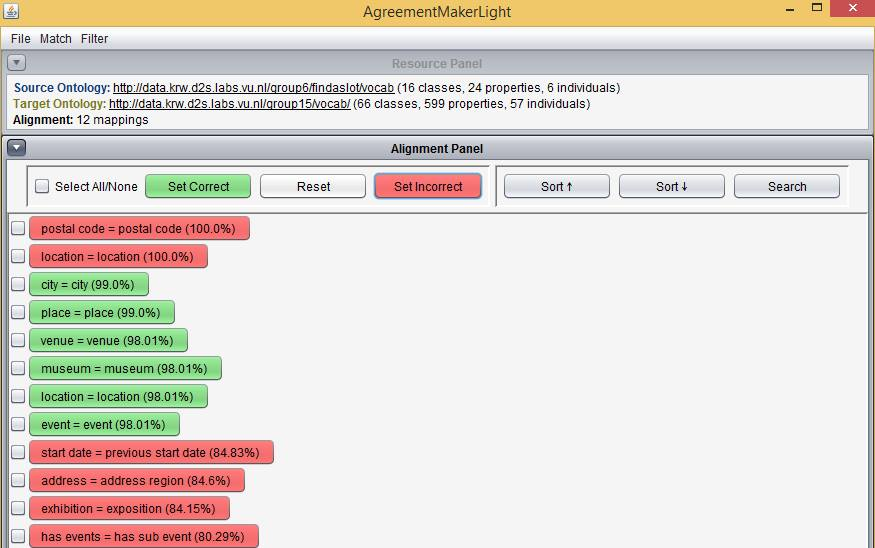
\includegraphics[width=.75\textwidth]{img/match_g15.png}
	\caption{Matching to group 15}
	\label{fig:match_g15}
\end{figure}



\section{Results and Discussion}
% Give here details about the most important results of your experiments. Use tables and figures, but focus on the interesting and important results. Make sure you describe in the text what the reviewers should see, explain what the reader sees in the tables and point to the interesting findings. Be explicit about your research question and hypothesis, and discuss they might be true, or false. 
- Led to ? 98\%  name comparison 99\% class comparison 100\%

- Intuitively, our ontology should have had more matches with group 10, since they model the exact same datasets as we do. However, they model the details of events as Entities, while we do it as Properties. To the best of our knowledge, AML cannot match entities to properties. This discovery raises more serious questions since the limitations of matching are evident when design decisions like the ones in this case rigidly prevent matches.

- Matches to ill formed ontologies are hard to predict. For example, Group 15 has two Venues entities which are matched to our single Venue entity in a cyclic way.

\section{Conclusion}
%Here you summarize the preceding sections, describe the lessons learnt and discuss future work.
- 
- Note: the field is messy and outdated tools are often referred.



\bibliographystyle{plain}
\bibliography{mybib}

\end{document}
